%%%%%%%%%%%%%%%%%%%%%%%%%%%%%%%%%%%%%%%%%%%%%%%%%%%%%%%%%%%%%%%%%%%%%%%
% Based on IEEE the conference template available                     %
% at https://www.ieee.org/conferences/publishing/templates.html       %
% Adapted for the Data Science Lab course at Politecnico di Torino    %
% by Giuseppe Attanasio, Flavio Giobergia                             %
% 2020, DataBase and Data Mining Group                                %
%%%%%%%%%%%%%%%%%%%%%%%%%%%%%%%%%%%%%%%%%%%%%%%%%%%%%%%%%%%%%%%%%%%%%%%

\documentclass[conference]{IEEEtran}
\usepackage{cite}
\usepackage{amsmath,amssymb,amsfonts}
\usepackage{algorithmic}
\usepackage{graphicx}
\usepackage{textcomp}
\usepackage{xcolor}

\usepackage{graphicx}
\graphicspath{ {./figures/} }

\usepackage{tabularx,ragged2e,booktabs,caption}
\usepackage{multirow}


\begin{document}

\title{Report title}

\author{\IEEEauthorblockN{Giulia Monchietto, Andrea Ruglioni}
\IEEEauthorblockA{\textit{Politecnico di Torino} \\
Student id: s123456, s123456\\
email@studenti.polito.it, email@studenti.polito.it}
}

\maketitle

\begin{abstract}
    In this report, a machine learning model for intent recognition is proposed.
    The model is able to recognize key words from wav audio files by using Mel-frequency cepstral coefficients (MFCCs) as features, Principal Component Analysis (PCA) to reduce features number, and K-Nearest Neighbors (KNN) algorithm as a classifier.
    It achieves an accuracy of 0.762 on the public leaderboard, showing potential for future improvements.
\end{abstract}

% \begin{figure}
%     \centering
%     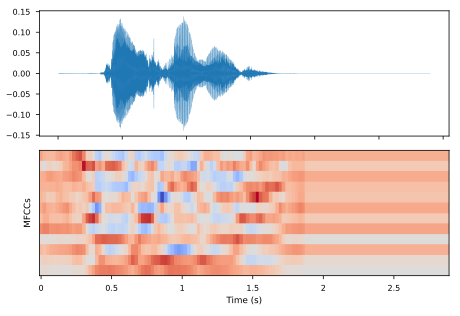
\includegraphics{m}
%     \caption{graph}
% \end{figure}

% \begin{figure}
%     \begin{subfigure}{.5\textwidth}
%         \input{figures/wave.pgf}
%         \caption{Subplot 1}
%     \end{subfigure}
%     \begin{subfigure}{.5\textwidth}
%         \input{figures/mfcc.pgf}
%         \caption{Subplot 2}
%     \end{subfigure}
% \end{figure}

\section{Problem overview}
Intent recognition is an important task in natural language processing (NLP) and speech recognition.
Its goal is to determine the underlying purpose of a part of speech.
This is a challenging task because the audio files contain little background noise and people speaking with different accents and variations in speaking style.
Additionally, audio data are not easy to work with as they require specialized preprocessing techniques in order to extract useful features.

The dataset given has been divided in two parts:
\begin{itemize}
    \item \textbf{Development} set, containing 9954 instances, 7 predictive attributes and the target, \textit{intent}.
    \item \textbf{Evaluation} set, containing 1455 instances with the same structure besides the target variable.
\end{itemize}
The split has been made in order to train a model using the first one, and evaluate its accuracy using the second one.

Each row of the dataset contains information about the person speaking, from his/her \textit{speakerId}, to his/her \textit{gender}, \textit{ageRange}, \textit{self-reported fluency level}, \textit{first Language spoken} and the \textit{current language used for work/school}, and the \textit{path} to the wav file.
The \textit{intent} refers to the purpose of the speaker and it is a categorical response variable assuming 7 possible values, some of which are "activate music", "increase heat" and "deactivate lights".

From a brief exploratory data analysis, it is immediate to observe that there are no missing or duplicated values. 
Then it can be noted that 10834 out of the total 11309 speakers are native english (from United States).
Thus, they account for nearly 96\% of the data, making the remaining speakers negligible and not numerically significant.
Therefore, we could cut off the 3 attributes regarding languages or alternatively consider the non native speakers as outliers and exclude them from the development set, focusing our attention to the recognition of the native ones intents.
Both options have been tested, bringing no significant difference in the results, so we will proceed with the first one.

On the other hand, \textit{gender} and \textit{ageRange} will be kept since speakers in the same bucket could have similar tone colour, making the recognition easier.

For what concerns the wav audio files, they have been sampled at the same rate, 22050 Hz, which is a standard value for speech recording when perceived quality is unimportant, but clarity must be maintained, providing a good trade-off between quality and memory load.
Moreover, the audio lengths are different, having a mean duration of about 2.6 seconds.
In order to extract an equal number of features from each recording, it will be necessary to properly adjust each one of them. 

Listening to some audios, it is interesting to note that the intent does not exactly coincide with the person statement.
For instance, the speaker could say "volume up" instead of "increase volume".
This increases the complexity of the problem because there is not temporal overlapping between speakers belonging to the same class.

\section{Proposed approach}
% The proposed approach for this task is to use Mel-frequency cepstral coefficients (MFCCs) as features, and Principal Component Analysis (PCA) to reduce the dimensionality.
% MFCCs are commonly used in speech recognition because they are a compact representation of the spectral envelope of the audio signal.
% They capture the unique characteristics of a speaker's voice and are robust to background noise.
% PCA is a technique used for feature extraction and dimensionality reduction, which can improve the computational efficiency of the model.
% The KNN algorithm is a simple, yet effective, classifier that can be useful for recognizing patterns in data.
% It works by comparing a given input to the k nearest examples in the training set, where k is a user-defined parameter.
\subsection{Preprocessing}

Firstly, the categorical features \textit{gender} and \textit{ageRange} have been one-hot-encoded (adding up respectively 2 and 3 features) while \textit{speakerId} has been discarded because it had 97 unique values.
Therefore, its encoding would have ramp the number of features up by 96, increasing the computational cost and time efficiency without actually improving the accuracy.

Moving our focus towards the audio files, they were preprocessed by trimming, cutting, and padding.
The first step involved removing any trailing and leading silences or background noises, making possible to cut the mean duration to about 1.8 seconds without any loss of relevant information.
Next, the audio files were cut and padded.
This has been done to ensure that the features extracted are comparable and of the same length, obtaining as a result consistent data for scikit-learn.
Going into detail, the 95th percentile $p$ of the lengths has been taken, indicating the length such that 95\% of data are shorter than $p$.
We got $p = 2.9$ seconds.
The cut and pad method refers, respectively, to the discard of the recording part over $p$ and to the addition of trailing zeros (which represent silence) to recording with length less than $p$.

The next step was to compute the Mel-frequency cepstral coefficients (MFCCs).
MFCCs are the “de facto” standard for speech recognition because of their high accuracy and low complexity.
However, they are not very robust at the presence of noise.
Therefore, it is common to normalise their values to lessen their influence, and so we did.
The term ceptral refers to the cepstrum, which is a tool to investigate periodic structures in frequency spectra.
Instead, Mel-frequency indicates that the frequency studied are equally spaced on the mel scale, which is a non-linear scale that is based on the way the human ear perceives different frequencies of sound.

At the end, Principal Component Analysis (PCA) was used to reduce the number of features.
In fact, the MFCC built from each recording is represented by a $125 \times 12$ matrix, prducing the overwhelming 1500 features plus the 5 from \textit{gender} and \textit{ageRange}.
PCA is a technique used for feature extraction and dimensionality reduction, which can improve the computational efficiency of the model.
It works by transforming the original features into a new set of features, called principal components, which are linear combinations of the original ones.
These principal components are chosen such that they capture the most important information in the original features, explaining the most variance possible.
In our case, narrow the features down to 272 still explaining the 90\% of the variance in the development set.

\subsection{Model selection}
The following two models have been deepened because researches have proved their efficiency for speech recognition systems:
\begin{itemize}
    \item The K-nearest neighbors (KNN) algorithm is a simple, yet effective, classifier that can be useful for recognizing patterns in data.
    It is a non-parametric method, which means it does not make any assumptions about the underlying data distribution.
    This makes it well-suited for a problem like intent recognition where the data may be very complex.
    Additionally, KNN algorithm is computationally efficient and easy to implement.

    \item The support vector machine (SVM) is a very versatile model whose basic idea is to find the best linear decision surface, that separates different classes.
    Their importance is due to the kernel trick, which vartually transforms the data in a higher dimensional space, where it is linearly separable, obtaining a non-linear decision boundary in the original feature space.
    For speech recognition models, SVMs are often used with a radial basis function (RBF) kernel.
    Moreover, with have trained SVM with a one vs one approach consisting in fitting one classifier per class pair.
    At prediction time, the class which receives the most votes is selected.
    Thus
\end{itemize}

\subsection{Hyperparameters tuning}
In this section is reported the tuning of the previous models' hyperparameters using a grid search 5-fold cross-validation method.
It involves training the model multiple times with different combinations of hyperparameters, and evaluating the performance of each combination using cross-validation.
In our case, the performance score of interest is the accuracy.
The possible parameters' values can be seen in table \ref{tab:grid}.

\begin{table}
    \centering
    \caption{parameters grid}
    \begin{tabular}{lllll}
        \toprule
        \toprule
        Models & Parameters & Values\\
        \midrule
        \addlinespace[5pt]
        \multirow{2}{*}[-3pt]{SVM}  & kernel & ['linear', 'poly', 'rbf']\\
                                    \cmidrule{2-3}
                                    & C      & [0.1, 1, 10]\\
        \midrule
        \multirow{2}{*}[-3pt]{KNN}  & n neighbors & [5, 6, 7, 8, 9, 10]\\
                                    \cmidrule{2-3}
                                    & weights     & ['uniform', 'distance']\\
        \bottomrule
    \end{tabular}
    \label{tab:grid}
\end{table}

In general $k$-fold cross-validation is a method of evaluating the performance by dividing the development data into training and validation sets, with size respectively $(k-1)/k$ and $1/k$.
This process is repeated $k$ times with different partitions of the data, and the average performance is used to evaluate the model.
Therefore, $k$ training and testing processes have to be made which could be computationally expensive for slow models.

\section{Results}

\begin{table}
    \centering
    \caption{results on public leaderboard}
    \begin{tabular}{lllll}
        \toprule
        \toprule
        Models & Accuracy & Best parameters \\
        \midrule
        \addlinespace[5pt]
        \multirow{2}{*}[-3pt]{SVM} & \multirow{2}{*}[-3pt]{0.728}   & kernel: 'rbf'\\
                                                                    \cmidrule{3-3}
                                                                    && C: 10\\
        \midrule
        \multirow{2}{*}[-3pt]{KNN} & \multirow{2}{*}[-3pt]{0.762}   & n neighbors: 6\\
                                                                    \cmidrule{3-3}
                                                                    && weights: 'distance'\\
        \bottomrule
    \end{tabular}
    \label{tab:results}
\end{table}

In this section we will show the results obtained using the procedures described in previous sections.
After model selection, KNN and SVM algorithms have been tested with the selected hyperparameters showed in Table \ref{tab:grid}.
For testing purpose k-fold cross validation on the development set has been used, leading to the average accuracies in Table \ref{tab:results_dev}.
\begin{table}
    \centering
    \caption{Results of hyperparameters tuning using k-fold cross validation}
    \begin{tabular}{lllll}
        \toprule
        \toprule
        Models & Accuracy & Best parameters \\
        \midrule
        \addlinespace[5pt]
        \multirow{2}{*}[-3pt]{SVM} & \multirow{2}{*}[-3pt]{0.639}   & kernel: 'rbf'\\
                                                                    \cmidrule{3-3}
                                                                    && C: 10\\
        \midrule
        \multirow{2}{*}[-3pt]{KNN} & \multirow{2}{*}[-3pt]{0.667}   & n neighbors: 6\\
                                                                    \cmidrule{3-3}
                                                                    && weights: 'distance'\\
        \bottomrule
    \end{tabular}
    \label{tab:results_dev}
\end{table}

The results show little difference in accuracy, with KNN algorithm performing slightly better.\\
Subsequently, we have validated our KNN algorithm with the best hyperparameters configuration found, changing features quality.
We have tested 6 different values for the MFCCs number hyperparameter: 8, 10, 12, 14, 16 and the default value 20. The optimal number found has been 10, with accuracy displayed in Table \ref{tab:results_n_mfcc}.\\
\begin{table}
    \centering
    \caption{Results of MFCCs number tuning on KNN}
    \begin{tabular}{lllll}
        \toprule
        \toprule
        MFCCs number & Accuracy \\
        \midrule
        \addlinespace[5pt]
        \multirow{2}{*}[-3pt]{8} & \multirow{2}{*}[-3pt]{0.66003}\\
        \multirow{2}{*}[-3pt]{10} & \multirow{2}{*}[-3pt]{0.66023}\\
        \multirow{2}{*}[-3pt]{12} & \multirow{2}{*}[-3pt]{0.65516}\\
        \multirow{2}{*}[-3pt]{14} & \multirow{2}{*}[-3pt]{0.65049}\\
        \multirow{2}{*}[-3pt]{16} & \multirow{2}{*}[-3pt]{0.63171}\\
        \multirow{2}{*}[-3pt]{20} & \multirow{2}{*}[-3pt]{0.60502}\\
        \bottomrule
    \end{tabular}
    \label{tab:results_n_mfcc}
\end{table}
After model selection and hyperparameters tuning processes, the two best models have been evaluated on the public evaluation test set.\\
The \textbf{SVM} model achieved an accuracy of \textbf{0.728}, while \textbf{KNN} model achieved an accuracy of \textbf{0.762}.


\section{Discussion}
The results demonstrate the potential of using MFCCs, PCA and KNN algorithm for intent recognition task.
The preprocessing steps and hyperparameter tuning were crucial for achieving good performance.
The results were compared with SVM model, which can be used as benchmark for future work.
In fact, inference for SVM model takes $O(d)$, where $d$ is the number of features, since you only need to determine which side of a hyperplane a given point lies on.
While KNN inference requires computation of distances between new objects and already classified objects.
Therefore for fast classification purposes SVM could help achieve a more efficient performance with sligtly worse accuracy results.


The results also indicate that there is room for improvement and further research could be done to improve the performance of the model.
For example, other feature extraction techniques or classifiers could be explored, and the model could be trained on a larger dataset to increase its generalizability.
Additionally, incorporating techniques like data augmentation and ensembling could help to further improve the performance.


\nocite{*}
\bibliography{bibliography}
\bibliographystyle{ieeetr}

\end{document}
